\documentclass[11pt]{article}
\usepackage[margin=1in]{geometry}
\usepackage{amsmath,amssymb}
\usepackage{graphicx}
\usepackage{booktabs}
\usepackage{longtable}
\usepackage{hyperref}
\usepackage{natbib}
\usepackage{xcolor}
\usepackage{microtype}
\usepackage[affil-it]{authblk}
\usepackage[section]{placeins}

\newcommand{\TODO}[1]{\textcolor{red}{[TODO: #1]}}

% Extra space before floats (matches pQTL/cross-ancestry papers)
\setlength{\textfloatsep}{14pt plus 2pt minus 2pt}
\setlength{\intextsep}{10pt plus 2pt minus 2pt}

\title{Only Two of Ten RNA and DNA Foundation Models Retain\\Base-Pairing Signal Under Composition-Matched Nulls}

\author{Elliot Tower}
\affil{Independent researcher \\ \texttt{elliot@elliottower.ai}}
\date{}

% Running head for RNA journal (<=50 chars):
% Base pairing under composition-matched nulls

% Panel counts and every reported number, written by
% scripts/generate_results_tables.py from the stamped runs.
% Generated by scripts/generate_panel_description.py. Do not edit.
% Every figure below is computed from data/rfam_families/.
\newcommand{\panelN}{47}
\newcommand{\panelCurated}{52}
\newcommand{\panelWithdrawn}{5}
\newcommand{\panelClasses}{riboswitches (14), cis-regulatory elements (8), other ncRNAs (8), ribozymes (6), miRNA precursors (4), snRNAs (4), tRNAs (2), and CRISPR repeats (1)}
\newcommand{\panelLengthRange}{30--387}
\newcommand{\panelLengthMedian}{106}
\newcommand{\panelLengthIQR}{77.5--166}
\newcommand{\panelStemGC}{59.1}
\newcommand{\panelLoopGC}{43.0}
\newcommand{\panelGCEnriched}{40}
\newcommand{\panelGCScored}{47}

% Written by scripts/generate_results_tables.py. Do not edit.
\newcommand{\confirmatoryN}{36}
\newcommand{\gateThreshold}{8}
\newcommand{\gateRegistered}{7}
\newcommand{\bootstrapB}{10{,}000}
\newcommand{\panelHashShort}{\texttt{5c4d6f6d4c32}}
\newcommand{\provenanceRuns}{17}
\newcommand{\provenanceCommits}{2}
\newcommand{\provenanceStacks}{5}
\newcommand{\ratioErnieRNA}{1.276}
\newcommand{\ciErnieRNA}{[1.22, 1.34]}
\newcommand{\exceedErnieRNA}{31}
\newcommand{\dinucErnieRNA}{30}
\newcommand{\retainErnieRNA}{30 of 31}
\newcommand{\retainPctErnieRNA}{97\%}
\newcommand{\probeErnieRNA}{0.683}
\newcommand{\probeDeltaErnieRNA}{+0.183}
\newcommand{\probeLayerErnieRNA}{11}
\newcommand{\attnErnieRNA}{0.113}
\newcommand{\psErnieRNA}{0.1113}
\newcommand{\gateErnieRNA}{34/36}
\newcommand{\gateCountErnieRNA}{34}
\newcommand{\eligibleErnieRNA}{36}
\newcommand{\nullErnieRNA}{32/34}
\newcommand{\consErnieRNA}{32/34}
\newcommand{\hthreeErnieRNA}{0.885}
\newcommand{\psPeakErnieRNA}{12}
\newcommand{\psLayersErnieRNA}{13}
\newcommand{\psPeakCountErnieRNA}{29 of 34}
\newcommand{\ratioRiNALMo}{1.143}
\newcommand{\ciRiNALMo}{[1.12, 1.17]}
\newcommand{\exceedRiNALMo}{17}
\newcommand{\dinucRiNALMo}{15}
\newcommand{\retainRiNALMo}{15 of 17}
\newcommand{\retainPctRiNALMo}{88\%}
\newcommand{\probeRiNALMo}{0.633}
\newcommand{\probeDeltaRiNALMo}{+0.133}
\newcommand{\probeLayerRiNALMo}{32}
\newcommand{\attnRiNALMo}{0.107}
\newcommand{\psRiNALMo}{0.2062}
\newcommand{\gateRiNALMo}{32/36}
\newcommand{\gateCountRiNALMo}{32}
\newcommand{\eligibleRiNALMo}{36}
\newcommand{\nullRiNALMo}{31/32}
\newcommand{\consRiNALMo}{29/32}
\newcommand{\hthreeRiNALMo}{0.886}
\newcommand{\psPeakRiNALMo}{33}
\newcommand{\psLayersRiNALMo}{34}
\newcommand{\psPeakCountRiNALMo}{31 of 32}
\newcommand{\ratioRNAFM}{1.722}
\newcommand{\ciRNAFM}{[1.53, 1.95]}
\newcommand{\exceedRNAFM}{0}
\newcommand{\dinucRNAFM}{0}
\newcommand{\probeRNAFM}{0.550}
\newcommand{\probeDeltaRNAFM}{+0.050}
\newcommand{\probeLayerRNAFM}{0}
\newcommand{\attnRNAFM}{0.049}
\newcommand{\psRNAFM}{$8.9 \times 10^{-5}$}
\newcommand{\gateRNAFM}{2/36}
\newcommand{\gateCountRNAFM}{2}
\newcommand{\eligibleRNAFM}{36}
\newcommand{\nullRNAFM}{0/2}
\newcommand{\consRNAFM}{0/2}
\newcommand{\hthreeRNAFM}{0.250}
\newcommand{\psPeakRNAFM}{1}
\newcommand{\psLayersRNAFM}{13}
\newcommand{\psPeakCountRNAFM}{1 of 2}
\newcommand{\ratioUTRLM}{1.056}
\newcommand{\ciUTRLM}{[1.04, 1.08]}
\newcommand{\exceedUTRLM}{3}
\newcommand{\dinucUTRLM}{2}
\newcommand{\retainUTRLM}{2 of 3}
\newcommand{\retainPctUTRLM}{67\%}
\newcommand{\probeUTRLM}{0.578}
\newcommand{\probeDeltaUTRLM}{+0.078}
\newcommand{\probeLayerUTRLM}{1}
\newcommand{\attnUTRLM}{0.051}
\newcommand{\psUTRLM}{$8.3 \times 10^{-6}$}
\newcommand{\gateUTRLM}{27/36}
\newcommand{\gateCountUTRLM}{27}
\newcommand{\eligibleUTRLM}{36}
\newcommand{\nullUTRLM}{18/27}
\newcommand{\consUTRLM}{4/27}
\newcommand{\hthreeUTRLM}{0.215}
\newcommand{\psPeakUTRLM}{0}
\newcommand{\psLayersUTRLM}{7}
\newcommand{\psPeakCountUTRLM}{15 of 27}
\newcommand{\ratioSpliceBERT}{1.040}
\newcommand{\ciSpliceBERT}{[1.03, 1.05]}
\newcommand{\exceedSpliceBERT}{3}
\newcommand{\dinucSpliceBERT}{1}
\newcommand{\retainSpliceBERT}{1 of 3}
\newcommand{\retainPctSpliceBERT}{33\%}
\newcommand{\probeSpliceBERT}{0.566}
\newcommand{\probeDeltaSpliceBERT}{+0.066}
\newcommand{\probeLayerSpliceBERT}{1}
\newcommand{\attnSpliceBERT}{0.054}
\newcommand{\psSpliceBERT}{0.0002}
\newcommand{\gateSpliceBERT}{25/36}
\newcommand{\gateCountSpliceBERT}{25}
\newcommand{\eligibleSpliceBERT}{36}
\newcommand{\nullSpliceBERT}{15/25}
\newcommand{\consSpliceBERT}{4/25}
\newcommand{\hthreeSpliceBERT}{0.270}
\newcommand{\psPeakSpliceBERT}{0}
\newcommand{\psLayersSpliceBERT}{7}
\newcommand{\psPeakCountSpliceBERT}{11 of 25}
\newcommand{\ratioNTvTwo}{1.113}
\newcommand{\ciNTvTwo}{[1.08, 1.14]}
\newcommand{\exceedNTvTwo}{15}
\newcommand{\dinucNTvTwo}{10}
\newcommand{\retainNTvTwo}{10 of 15}
\newcommand{\retainPctNTvTwo}{67\%}
\newcommand{\probeNTvTwo}{0.531}
\newcommand{\probeDeltaNTvTwo}{+0.031}
\newcommand{\probeLayerNTvTwo}{7}
\newcommand{\attnNTvTwo}{0.242}
\newcommand{\psNTvTwo}{0.0014}
\newcommand{\gateNTvTwo}{1/4}
\newcommand{\gateCountNTvTwo}{1}
\newcommand{\eligibleNTvTwo}{4}
\newcommand{\nullNTvTwo}{0/1}
\newcommand{\consNTvTwo}{0/1}
\newcommand{\hthreeNTvTwo}{0.500}
\newcommand{\psPeakNTvTwo}{0}
\newcommand{\psLayersNTvTwo}{13}
\newcommand{\psPeakCountNTvTwo}{1 of 1}
\newcommand{\ratioDNABERTTwo}{1.003}
\newcommand{\ciDNABERTTwo}{[0.97, 1.04]}
\newcommand{\exceedDNABERTTwo}{8}
\newcommand{\dinucDNABERTTwo}{5}
\newcommand{\retainDNABERTTwo}{5 of 8}
\newcommand{\retainPctDNABERTTwo}{62\%}
\newcommand{\probeDNABERTTwo}{0.530}
\newcommand{\probeDeltaDNABERTTwo}{+0.030}
\newcommand{\probeLayerDNABERTTwo}{1}
\newcommand{\attnDNABERTTwo}{0.199}
\newcommand{\psDNABERTTwo}{-0.0680}
\newcommand{\gateDNABERTTwo}{0/8}
\newcommand{\gateCountDNABERTTwo}{0}
\newcommand{\eligibleDNABERTTwo}{8}
\newcommand{\ratioHyenaDNA}{1.160}
\newcommand{\ciHyenaDNA}{[1.12, 1.20]}
\newcommand{\exceedHyenaDNA}{8}
\newcommand{\dinucHyenaDNA}{7}
\newcommand{\retainHyenaDNA}{7 of 8}
\newcommand{\retainPctHyenaDNA}{88\%}
\newcommand{\probeHyenaDNA}{0.577}
\newcommand{\probeDeltaHyenaDNA}{+0.077}
\newcommand{\probeLayerHyenaDNA}{0}
\newcommand{\psHyenaDNA}{0.0002}
\newcommand{\gateHyenaDNA}{27/36}
\newcommand{\gateCountHyenaDNA}{27}
\newcommand{\eligibleHyenaDNA}{36}
\newcommand{\nullHyenaDNA}{13/27}
\newcommand{\consHyenaDNA}{6/27}
\newcommand{\hthreeHyenaDNA}{0.162}
\newcommand{\psPeakHyenaDNA}{0}
\newcommand{\psLayersHyenaDNA}{4}
\newcommand{\psPeakCountHyenaDNA}{26 of 27}
\newcommand{\ratioCaduceus}{1.206}
\newcommand{\ciCaduceus}{[1.16, 1.26]}
\newcommand{\exceedCaduceus}{8}
\newcommand{\dinucCaduceus}{4}
\newcommand{\retainCaduceus}{4 of 8}
\newcommand{\retainPctCaduceus}{50\%}
\newcommand{\probeCaduceus}{0.577}
\newcommand{\probeDeltaCaduceus}{+0.077}
\newcommand{\probeLayerCaduceus}{0}
\newcommand{\psCaduceus}{0.0039}
\newcommand{\gateCaduceus}{18/36}
\newcommand{\gateCountCaduceus}{18}
\newcommand{\eligibleCaduceus}{36}
\newcommand{\nullCaduceus}{13/18}
\newcommand{\consCaduceus}{8/18}
\newcommand{\hthreeCaduceus}{0.402}
\newcommand{\psPeakCaduceus}{3}
\newcommand{\psLayersCaduceus}{17}
\newcommand{\psPeakCountCaduceus}{4 of 18}
\newcommand{\ratioEvo}{1.450}
\newcommand{\ciEvo}{[1.30, 1.63]}
\newcommand{\exceedEvo}{8}
\newcommand{\dinucEvo}{6}
\newcommand{\retainEvo}{6 of 8}
\newcommand{\retainPctEvo}{75\%}
\newcommand{\probeEvo}{0.552}
\newcommand{\probeDeltaEvo}{+0.052}
\newcommand{\probeLayerEvo}{0}
\newcommand{\psEvo}{0.0017}
\newcommand{\gateEvo}{13/36}
\newcommand{\gateCountEvo}{13}
\newcommand{\eligibleEvo}{36}
\newcommand{\nullEvo}{6/13}
\newcommand{\consEvo}{2/13}
\newcommand{\hthreeEvo}{0.376}
\newcommand{\psPeakEvo}{12}
\newcommand{\psLayersEvo}{32}
\newcommand{\psPeakCountEvo}{7 of 13}
\newcommand{\exceedUntrainedErnieRNA}{2}
\newcommand{\ratioUntrainedErnieRNA}{1.815}
\newcommand{\retainUntrainedErnieRNA}{2 of 2}
\newcommand{\attnUntrainedErnieRNA}{0.085}
\newcommand{\attnDeltaErnieRNA}{+0.027}
\newcommand{\attnFamilyDeltaErnieRNA}{+0.027}
\newcommand{\attnHigherTrainedErnieRNA}{47}
\newcommand{\attnHigherUntrainedErnieRNA}{0}
\newcommand{\psUntrainedErnieRNA}{$6.0 \times 10^{-9}$}
\newcommand{\gateUntrainedErnieRNA}{6/36}
\newcommand{\nullUntrainedErnieRNA}{4/6}
\newcommand{\signErnieRNA}{7/47}
\newcommand{\signPctErnieRNA}{15\%}
\newcommand{\exceedUntrainedRiNALMo}{5}
\newcommand{\ratioUntrainedRiNALMo}{4.556}
\newcommand{\retainUntrainedRiNALMo}{1 of 5}
\newcommand{\attnUntrainedRiNALMo}{0.064}
\newcommand{\attnDeltaRiNALMo}{+0.044}
\newcommand{\attnFamilyDeltaRiNALMo}{+0.044}
\newcommand{\attnHigherTrainedRiNALMo}{46}
\newcommand{\attnHigherUntrainedRiNALMo}{1}
\newcommand{\psUntrainedRiNALMo}{$1.1 \times 10^{-8}$}
\newcommand{\gateUntrainedRiNALMo}{6/36}
\newcommand{\nullUntrainedRiNALMo}{4/6}
\newcommand{\signRiNALMo}{0/47}
\newcommand{\signPctRiNALMo}{0\%}
\newcommand{\exceedUntrainedRNAFM}{2}
\newcommand{\ratioUntrainedRNAFM}{2.257}
\newcommand{\retainUntrainedRNAFM}{1 of 2}
\newcommand{\attnUntrainedRNAFM}{0.043}
\newcommand{\attnDeltaRNAFM}{+0.006}
\newcommand{\attnFamilyDeltaRNAFM}{+0.006}
\newcommand{\attnHigherTrainedRNAFM}{33}
\newcommand{\attnHigherUntrainedRNAFM}{14}
\newcommand{\psUntrainedRNAFM}{$4.5 \times 10^{-9}$}
\newcommand{\gateUntrainedRNAFM}{9/36}
\newcommand{\nullUntrainedRNAFM}{5/9}
\newcommand{\signRNAFM}{17/47}
\newcommand{\signPctRNAFM}{36\%}
\newcommand{\exceedUntrainedUTRLM}{1}
\newcommand{\ratioUntrainedUTRLM}{1.038}
\newcommand{\retainUntrainedUTRLM}{0 of 1}
\newcommand{\attnUntrainedUTRLM}{0.054}
\newcommand{\attnDeltaUTRLM}{-0.003}
\newcommand{\attnFamilyDeltaUTRLM}{-0.003}
\newcommand{\attnHigherTrainedUTRLM}{16}
\newcommand{\attnHigherUntrainedUTRLM}{31}
\newcommand{\psUntrainedUTRLM}{$-2.0 \times 10^{-8}$}
\newcommand{\gateUntrainedUTRLM}{4/36}
\newcommand{\nullUntrainedUTRLM}{0/4}
\newcommand{\signUTRLM}{31/47}
\newcommand{\signPctUTRLM}{66\%}
\newcommand{\exceedUntrainedSpliceBERT}{4}
\newcommand{\ratioUntrainedSpliceBERT}{1.238}
\newcommand{\retainUntrainedSpliceBERT}{4 of 4}
\newcommand{\attnUntrainedSpliceBERT}{0.032}
\newcommand{\attnDeltaSpliceBERT}{+0.022}
\newcommand{\attnFamilyDeltaSpliceBERT}{+0.022}
\newcommand{\attnHigherTrainedSpliceBERT}{45}
\newcommand{\attnHigherUntrainedSpliceBERT}{2}
\newcommand{\psUntrainedSpliceBERT}{$7.1 \times 10^{-10}$}
\newcommand{\gateUntrainedSpliceBERT}{9/36}
\newcommand{\nullUntrainedSpliceBERT}{5/9}
\newcommand{\signSpliceBERT}{10/47}
\newcommand{\signPctSpliceBERT}{21\%}
\newcommand{\exceedUntrainedNTvTwo}{10}
\newcommand{\ratioUntrainedNTvTwo}{1.037}
\newcommand{\retainUntrainedNTvTwo}{9 of 10}
\newcommand{\attnUntrainedNTvTwo}{0.246}
\newcommand{\attnDeltaNTvTwo}{-0.004}
\newcommand{\attnFamilyDeltaNTvTwo}{-0.004}
\newcommand{\attnHigherTrainedNTvTwo}{23}
\newcommand{\attnHigherUntrainedNTvTwo}{24}
\newcommand{\psUntrainedNTvTwo}{$-7.5 \times 10^{-9}$}
\newcommand{\gateUntrainedNTvTwo}{1/4}
\newcommand{\nullUntrainedNTvTwo}{0/1}
\newcommand{\signNTvTwo}{40/47}
\newcommand{\signPctNTvTwo}{85\%}
\newcommand{\exceedUntrainedDNABERTTwo}{6}
\newcommand{\ratioUntrainedDNABERTTwo}{8.416}
\newcommand{\retainUntrainedDNABERTTwo}{4 of 6}
\newcommand{\attnUntrainedDNABERTTwo}{0.190}
\newcommand{\attnDeltaDNABERTTwo}{+0.009}
\newcommand{\attnFamilyDeltaDNABERTTwo}{+0.009}
\newcommand{\attnHigherTrainedDNABERTTwo}{27}
\newcommand{\attnHigherUntrainedDNABERTTwo}{20}
\newcommand{\psUntrainedDNABERTTwo}{-0.0026}
\newcommand{\gateUntrainedDNABERTTwo}{2/8}
\newcommand{\nullUntrainedDNABERTTwo}{0/2}
\newcommand{\signDNABERTTwo}{27/47}
\newcommand{\signPctDNABERTTwo}{57\%}
\newcommand{\domainRankBiserial}{+0.04}
\newcommand{\domainP}{1.000}
\newcommand{\familiesScored}{47}
\newcommand{\expectedFalsePositives}{2.4}
\newcommand{\tuPerFamilyRNAFM}{0.93}
\newcommand{\tuOfMeansRNAFM}{0.76}
\newcommand{\tuPerFamilyRiNALMo}{0.50}
\newcommand{\tuOfMeansRiNALMo}{0.25}
\newcommand{\tuPerFamilySpliceBERT}{0.87}
\newcommand{\tuOfMeansSpliceBERT}{0.84}
\newcommand{\transversionAlphabet}{A$\to$C, C$\to$A, G$\to$U, U$\to$C}
\newcommand{\transErnieRNA}{1.253}
\newcommand{\transDeltaErnieRNA}{-1.7\%}
\newcommand{\transRiNALMo}{1.144}
\newcommand{\transDeltaRiNALMo}{+0.1\%}
\newcommand{\transRNAFM}{1.701}
\newcommand{\transDeltaRNAFM}{-1.2\%}
\newcommand{\transUTRLM}{1.058}
\newcommand{\transDeltaUTRLM}{+0.2\%}
\newcommand{\transSpliceBERT}{1.051}
\newcommand{\transDeltaSpliceBERT}{+1.0\%}
\newcommand{\transNTvTwo}{1.124}
\newcommand{\transDeltaNTvTwo}{+1.0\%}
\newcommand{\transDNABERTTwo}{0.988}
\newcommand{\transDeltaDNABERTTwo}{-1.5\%}
\newcommand{\transHyenaDNA}{1.073}
\newcommand{\transDeltaHyenaDNA}{-7.5\%}
\newcommand{\transCaduceus}{1.158}
\newcommand{\transDeltaCaduceus}{-4.0\%}
\newcommand{\transEvo}{1.465}
\newcommand{\transDeltaEvo}{+1.0\%}
\newcommand{\transversionWidest}{HyenaDNA}
\newcommand{\transversionWidestDeviation}{7.5\%}
\newcommand{\transversionBound}{8\%}
\newcommand{\attnBound}{0.05}
\newcommand{\attnWidest}{RiNALMo}
\newcommand{\attnWidestFactor}{1.7}
\newcommand{\psSeparation}{29}

% Written by scripts/generate_arm_tables.py. Do not edit.
\newcommand{\synPSRiNALMo}{0.0919}
\newcommand{\synPSDropRiNALMo}{55\%}
\newcommand{\synExcessRiNALMo}{+0.582}
\newcommand{\natExcessRiNALMo}{+0.770}
\newcommand{\synRetainedRiNALMo}{76\%}
\newcommand{\synPSErnieRNA}{0.0415}
\newcommand{\synPSDropErnieRNA}{63\%}
\newcommand{\synExcessErnieRNA}{+0.574}
\newcommand{\natExcessErnieRNA}{+0.764}
\newcommand{\synRetainedErnieRNA}{75\%}
\newcommand{\synN}{195}
\newcommand{\synPerFamily}{5}

% Written by scripts/layer_selection_audit.py. Do not edit.
\newcommand{\selectionDepthRho}{+0.12}
\newcommand{\selectionDepthP}{0.70}
\newcommand{\selectionArms}{13}
\newcommand{\selLayersErnieRNA}{13}
\newcommand{\selChanceErnieRNA}{0.124}
\newcommand{\selPerFamilyErnieRNA}{0.888}
\newcommand{\selPanelErnieRNA}{0.887}
\newcommand{\selHeldOutErnieRNA}{0.885}
\newcommand{\selHeldOutCIErnieRNA}{[0.814, 0.955]}
\newcommand{\selExcessErnieRNA}{0.764}
\newcommand{\selVsThirdErnieRNA}{0.555}
\newcommand{\selLayersRiNALMo}{34}
\newcommand{\selChanceRiNALMo}{0.102}
\newcommand{\selPerFamilyRiNALMo}{0.872}
\newcommand{\selPanelRiNALMo}{0.881}
\newcommand{\selHeldOutRiNALMo}{0.882}
\newcommand{\selHeldOutCIRiNALMo}{[0.822, 0.941]}
\newcommand{\selExcessRiNALMo}{0.770}
\newcommand{\selVsThirdRiNALMo}{0.538}
\newcommand{\selLayersCaduceus}{17}
\newcommand{\selChanceCaduceus}{0.218}
\newcommand{\selPerFamilyCaduceus}{0.340}
\newcommand{\selPanelCaduceus}{0.000}
\newcommand{\selHeldOutCaduceus}{0.002}
\newcommand{\selHeldOutCICaduceus}{[0.000, 0.000]}
\newcommand{\selExcessCaduceus}{0.122}
\newcommand{\selVsThirdCaduceus}{0.007}
\newcommand{\selLayersRNAFM}{13}
\newcommand{\selChanceRNAFM}{0.261}
\newcommand{\selPerFamilyRNAFM}{0.370}
\newcommand{\selPanelRNAFM}{0.124}
\newcommand{\selHeldOutRNAFM}{0.126}
\newcommand{\selHeldOutCIRNAFM}{[0.078, 0.175]}
\newcommand{\selExcessRNAFM}{0.109}
\newcommand{\selVsThirdRNAFM}{0.036}
\newcommand{\selLayersEvo}{32}
\newcommand{\selChanceEvo}{0.316}
\newcommand{\selPerFamilyEvo}{0.356}
\newcommand{\selPanelEvo}{0.314}
\newcommand{\selHeldOutEvo}{0.316}
\newcommand{\selHeldOutCIEvo}{[0.232, 0.402]}
\newcommand{\selExcessEvo}{0.040}
\newcommand{\selVsThirdEvo}{0.022}
\newcommand{\selLayersSpliceBERT}{7}
\newcommand{\selChanceSpliceBERT}{0.238}
\newcommand{\selPerFamilySpliceBERT}{0.247}
\newcommand{\selPanelSpliceBERT}{0.203}
\newcommand{\selHeldOutSpliceBERT}{0.203}
\newcommand{\selHeldOutCISpliceBERT}{[0.147, 0.257]}
\newcommand{\selExcessSpliceBERT}{0.009}
\newcommand{\selVsThirdSpliceBERT}{0.087}
\newcommand{\selLayersUTRLM}{7}
\newcommand{\selChanceUTRLM}{0.230}
\newcommand{\selPerFamilyUTRLM}{0.246}
\newcommand{\selPanelUTRLM}{0.191}
\newcommand{\selHeldOutUTRLM}{0.191}
\newcommand{\selHeldOutCIUTRLM}{[0.130, 0.250]}
\newcommand{\selExcessUTRLM}{0.016}
\newcommand{\selVsThirdUTRLM}{0.087}
\newcommand{\selLayersHyenaDNA}{4}
\newcommand{\selChanceHyenaDNA}{0.148}
\newcommand{\selPerFamilyHyenaDNA}{0.138}
\newcommand{\selPanelHyenaDNA}{0.122}
\newcommand{\selHeldOutHyenaDNA}{0.121}
\newcommand{\selHeldOutCIHyenaDNA}{[0.067, 0.177]}
\newcommand{\selExcessHyenaDNA}{-0.010}
\newcommand{\selVsThirdHyenaDNA}{0.195}
\newcommand{\selLayersErnieRNAUntrained}{13}
\newcommand{\selChanceErnieRNAUntrained}{0.241}
\newcommand{\selPerFamilyErnieRNAUntrained}{0.490}
\newcommand{\selPanelErnieRNAUntrained}{0.479}
\newcommand{\selHeldOutErnieRNAUntrained}{0.478}
\newcommand{\selHeldOutCIErnieRNAUntrained}{[0.396, 0.557]}
\newcommand{\selExcessErnieRNAUntrained}{0.249}
\newcommand{\selVsThirdErnieRNAUntrained}{0.157}
\newcommand{\selLayersRiNALMoUntrained}{34}
\newcommand{\selChanceRiNALMoUntrained}{0.232}
\newcommand{\selPerFamilyRiNALMoUntrained}{0.337}
\newcommand{\selPanelRiNALMoUntrained}{0.158}
\newcommand{\selHeldOutRiNALMoUntrained}{0.157}
\newcommand{\selHeldOutCIRiNALMoUntrained}{[0.107, 0.209]}
\newcommand{\selExcessRiNALMoUntrained}{0.105}
\newcommand{\selVsThirdRiNALMoUntrained}{0.003}
\newcommand{\selLayersRNAFMUntrained}{13}
\newcommand{\selChanceRNAFMUntrained}{0.230}
\newcommand{\selPerFamilyRNAFMUntrained}{0.323}
\newcommand{\selPanelRNAFMUntrained}{0.143}
\newcommand{\selHeldOutRNAFMUntrained}{0.144}
\newcommand{\selHeldOutCIRNAFMUntrained}{[0.093, 0.196]}
\newcommand{\selExcessRNAFMUntrained}{0.093}
\newcommand{\selVsThirdRNAFMUntrained}{0.010}
\newcommand{\selLayersSpliceBERTUntrained}{7}
\newcommand{\selChanceSpliceBERTUntrained}{0.194}
\newcommand{\selPerFamilySpliceBERTUntrained}{0.210}
\newcommand{\selPanelSpliceBERTUntrained}{0.172}
\newcommand{\selHeldOutSpliceBERTUntrained}{0.172}
\newcommand{\selHeldOutCISpliceBERTUntrained}{[0.123, 0.221]}
\newcommand{\selExcessSpliceBERTUntrained}{0.016}
\newcommand{\selVsThirdSpliceBERTUntrained}{0.124}
\newcommand{\selLayersUTRLMUntrained}{7}
\newcommand{\selChanceUTRLMUntrained}{0.127}
\newcommand{\selPerFamilyUTRLMUntrained}{0.139}
\newcommand{\selPanelUTRLMUntrained}{0.132}
\newcommand{\selHeldOutUTRLMUntrained}{0.131}
\newcommand{\selHeldOutCIUTRLMUntrained}{[0.082, 0.181]}
\newcommand{\selExcessUTRLMUntrained}{0.011}
\newcommand{\selVsThirdUTRLMUntrained}{0.194}
\newcommand{\selMaxShiftPositive}{0.010}


\begin{document}
\maketitle

\noindent\textbf{Keywords:} RNA foundation models, secondary structure, composition confound, partner specificity, evaluation framework

% ============================================================================
% ABSTRACT — ~200 words
% Sequence: problem, design, primary result, positive result, replication,
%           interpretation, scope
% ============================================================================
\begin{abstract}
Evaluating whether RNA foundation models encode base-pairing structure requires
separating learned representation from nucleotide composition. Stems are GC-rich
and loops are AU-rich, so any composition-sensitive embedding inherits that
enrichment as apparent structure awareness. We apply a three-rung ladder to ten
RNA- and DNA-pretrained models across \panelN{} Rfam families. A
nucleotide-stratified null absorbs most of the apparent signal at Rung~1; a
dinucleotide-preserving null at Rung~2 leaves ERNIE-RNA with 30 families and
RiNALMo with 15, and every other model with fewer than nine. At Rung~3 a
mutation must perturb its base-pairing partner more than that partner's own stem
neighbors, measured against a null that permutes partner assignments within
each stem. Two models resolve which position pairs with which: RiNALMo at
$\selPerFamilyRiNALMo{}$ per-pair precision and ERNIE-RNA at
$\selPerFamilyErnieRNA{}$, where that null puts chance at
$\selChanceRiNALMo{}$ and $\selChanceErnieRNA{}$. Precision is read at the
layer maximizing mean PS within each family; choosing that layer on families
that do not report the number leaves RiNALMo at $\selHeldOutRiNALMo{}$ and
ERNIE-RNA at $\selHeldOutErnieRNA{}$ and places the other eight models at or
below their own chance rates. Pretraining domain does not order
those eight: Evo at 7B parameters and RNA-FM at 99M sit with the
DNA-pretrained models.
A randomly initialized ERNIE-RNA clears every rung, reaching $0.490$ per-pair
precision. Its architecture holds a hardcoded Watson--Crick table in a buffer
that weight randomization does not reach; ablating it drops the randomly
initialized model to its own chance rate, $+0.012$ excess, while the trained
model retains $+0.725$.
\end{abstract}

% ============================================================================
% INTRODUCTION — 5 paragraphs, ~800 words
% Sequence: why it matters, confound, gap, what we do, contributions
% ============================================================================
\section{Introduction}
\label{sec:intro}

% P1: Why this matters
RNA foundation models are routinely claimed to encode secondary structure,
but the evaluation methods---downstream task performance, linear probing,
mutation sensitivity, attention--contact correlation---each answer different
questions, and none controls for sequence composition. Deep learning models
for RNA structure prediction may fail to generalize across families
\citep{szikszai2022generalization}; whether the same fragility applies to
learned representations has received less scrutiny.

% P2: The specific confound
Stems and loops differ in sequence composition. Across \panelN{} Rfam families,
stems average \panelStemGC{}\% G/C content while loops average
\panelLoopGC{}\%, and stem G/C exceeds loop G/C in \panelGCEnriched{} of
\panelGCScored{} families (Figure~\ref{fig:composition}). Because complement swaps at G/C positions
produce inherently larger embedding perturbations than at A/U positions,
any naive stem-versus-loop comparison inherits this enrichment. A
representation can therefore separate stems from loops without encoding
pairing topology.

% P3: The gap
Each evaluation method inherits the composition confound differently.
Linear probes can classify stems from loops using GC content alone.
Mutation sensitivity ratios conflate the larger perturbation magnitude at
G/C sites with structural relevance. Attention--contact correlations
bypass embeddings entirely and so measure a different channel. To
distinguish composition sensitivity from structure awareness, an
evaluation must control for nucleotide identity while testing whether
perturbations propagate to specific pairing partners.

% P4: What this study does — rung framing
These observations motivate a graded evaluation.
``Structure awareness'' encompasses at least three levels of
resolution, each demanding stronger knowledge: (1)~stem-versus-loop
discrimination, achievable by any representation sensitive to
nucleotide composition; (2)~discrimination surviving composition
controls at one and two orders of sequence context; and (3)~knowing
which specific position pairs with which, requiring that the model
encode the pairing topology. We apply this three-rung ladder to ten models across five architectures
and three orders of magnitude in parameter count.

% P5: Contributions + closing
The evaluation reveals a surprising asymmetry: the hardest test
produces the clearest positive result. Two RNA-pretrained
models---ERNIE-RNA (86M, with an architectural base-pairing attention
bias) and RiNALMo (650M, standard attention)---clear Rung~3 with
partner specificity two orders of magnitude above all other models,
while the remaining eight produce near-zero signal. We contribute:
(1)~a composition-controlled perturbation evaluation for RNA
foundation models; (2)~a ten-model benchmark with randomized-weight
controls on \panelN{} Rfam families; and (3)~evidence that two models
retain partner-specific pairing responses after composition controls are
applied.


% ============================================================================
% RESULTS — inferential logic: confound first, positive result, replication,
%           robustness, HTT last
% ============================================================================
\section{Results}

\subsection{Composition creates apparent structure signal (Rungs 1--2)}
\label{sec:composition-results}

Mutating a position to its Watson--Crick complement perturbs stem positions
more than loop positions in nine of ten models, with mean ratios from
$\ratioRNAFM{}$ (RNA-FM) down to near unity (Table~\ref{tab:rung1}). Stems in
this panel are GC-rich and loops are AU-rich---mean stem GC $\panelStemGC{}\%$
against loop GC $\panelLoopGC{}\%$---so a ratio above one is what a
composition-sensitive embedding produces whether or not it represents pairing.

Against a null that permutes stem and loop labels within nucleotide strata, most
of that signal is absorbed. At $\alpha = 0.05$ per family, chance alone places
2.4 of $\panelN{}$ families above the 95th percentile. ERNIE-RNA exceeds it in
$\exceedErnieRNA{}$ families and RiNALMo in $\exceedRiNALMo{}$; RNA-FM, whose
raw ratio is the largest in the panel, exceeds it in $\exceedRNAFM{}$.

A ratio and a composition-controlled count therefore order the models
differently, and neither distinguishes a model that tracks pairing from one that
tracks the nucleotides pairing implies. Rung 2 tightens the null to preserve
dinucleotide composition; Rung 3 changes the question.

\begin{figure}[htbp]
\centering
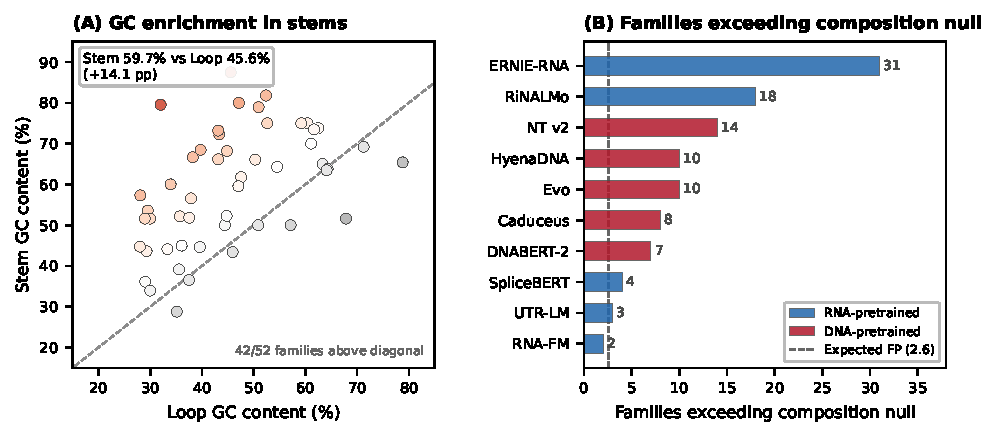
\includegraphics[width=\textwidth]{../figures/figure2_composition.pdf}
\caption{Composition confound. (A)~Stem GC content exceeds loop GC content
in \panelGCEnriched{} of \panelGCScored{} families (mean stem GC
\panelStemGC{}\% against loop GC \panelLoopGC{}\%). (B)~Number
of families per model whose stem--loop sensitivity ratio exceeds the
nucleotide-stratified null at the 95th percentile; dashed line marks the
expected false-positive count under independence
($m \times \alpha = \expectedFalsePositives{}$).
ERNIE-RNA (31) and RiNALMo (18) retain the most signal after composition
control.}
\label{fig:composition}
\end{figure}


\subsection{Probe validation}
\label{sec:probe-validation}

Eight of ten models score at their own chance rate at Rung 3, which admits two
readings the panel cannot separate, since every arm in it is a model under test.
We therefore run the Rung 3 procedure unchanged on two constructed embeddings
whose answer is fixed in advance. In the oracle, each position's representation
is a function of its own nucleotide and its partner's; in the local control, of
its own nucleotide and its two sequence neighbors.

The oracle reaches per-pair precision $1.000$ against a derangement chance rate
of $0.099$. The local control reaches $0.155$ against $0.173$. Both use the same
statistic, the same null and the same code path as every model in
Table~\ref{tab:rung3}, over the $\chanceRateN{}$ families of the Rung 3
analysis set.

The two chance rates differ, $0.099$ and $0.173$, on systems whose answers are
known.

\subsection{Partner specificity separates two models (Rung 3)}
\label{sec:ps-results}

\begin{table}[htbp]
\centering
\caption{Mutation sensitivity across ten models on the repaired panel
($N = \panelN{}$ Rfam families). Bootstrap 95\% CIs on the mean ratio
resample per-family ratios ($B = 10{,}000$).
At $\alpha = 0.05$ per family, 2.4 of 47
families are expected to exceed the null by chance. Attention $\rho$ is the mean
best-head-best-layer Spearman correlation between symmetrized attention and the
contact map, and is undefined for the three state-space models. Probing $\Delta$
is balanced accuracy minus 0.5. Untrained rows randomize every weight at a fixed
seed and load through the same adapter as the trained row above them.}
\label{tab:rung1}
\small
\begin{tabular}{lrlccc}
\toprule
\textbf{Model} & \textbf{Mean ratio} & \textbf{95\% CI} & \textbf{Fam $>$ null} & \textbf{Attn $\rho$} & \textbf{Probing $\Delta$} \\
\midrule
ERNIE-RNA (86M, RNA)       & 1.276 & [1.22, 1.34] & 31/47 & 0.113 & $+0.183$ \\
RiNALMo (650M, RNA)        & 1.143 & [1.12, 1.17] & 17/47 & 0.107 & $+0.134$ \\
RNA-FM (99M, RNA)          & 1.741 & [1.53, 1.98] & 0/47 & 0.048 & $+0.050$ \\
UTR-LM ($\sim$2M, RNA)     & 1.056 & [1.04, 1.08] & 3/47 & 0.051 & $+0.078$ \\
SpliceBERT (19M, RNA)      & 1.040 & [1.03, 1.05] & 3/47 & 0.054 & $+0.066$ \\
NT~v2 (56M, DNA)           & 1.098 & [1.08, 1.12] & 9/47 & 0.234 & $+0.036$ \\
DNABERT-2 (117M, DNA)      & 0.996 & [0.98, 1.01] & 3/47 & 0.196 & $+0.051$ \\
HyenaDNA (5.4M, DNA)       & 1.160 & [1.12, 1.20] & 8/47 & --- & $+0.077$ \\
Caduceus (14M, DNA)        & 1.206 & [1.16, 1.26] & 8/47 & --- & $+0.077$ \\
Evo (7B, DNA)              & 1.458 & [1.30, 1.64] & 8/47 & --- & $+0.052$ \\
\midrule
ERNIE-RNA untrained        & 1.164 & [1.12, 1.21] & 10/47 & 0.085 & $+0.044$ \\
RiNALMo untrained          & 1.156 & [1.13, 1.19] & 10/47 & 0.064 & $+0.077$ \\
RNA-FM untrained           & 1.043 & [1.04, 1.05] & 3/47 & 0.043 & $+0.073$ \\
UTR-LM untrained           & 1.038 & [1.03, 1.04] & 1/47 & 0.054 & $+0.077$ \\
SpliceBERT untrained       & 1.054 & [1.04, 1.07] & 0/47 & 0.032 & $+0.070$ \\
NT~v2 untrained            & 1.015 & [1.01, 1.02] & 5/47 & 0.241 & $+0.025$ \\
DNABERT-2 untrained        & 33.880 & [0.95, 93.92] & 6/47 & 0.153 & $+0.011$ \\
\bottomrule
\end{tabular}
\end{table}


\begin{table}[htbp]
\centering
\caption{Dinucleotide-stratified null across all models on the repaired panel.
``Fam $>$ nuc'' counts families exceeding the nucleotide-stratified null;
``Survive dinuc'' counts how many of those also exceed the
dinucleotide-stratified null, which is computed only where the first-order null
is exceeded. Retention is the second count over the first, and its bootstrap
95\% CI resamples the families in the first.}
\label{tab:rung2}
\small
\begin{tabular}{lrrll}
\toprule
\textbf{Model} & \textbf{Fam $>$ nuc} & \textbf{Survive dinuc} & \textbf{Retention} & \textbf{95\% CI} \\
\midrule
ERNIE-RNA (86M, RNA)       & 31 & 30 & 97\% & [0.90, 1.00] \\
RiNALMo (650M, RNA)        & 17 & 15 & 88\% & [0.71, 1.00] \\
NT~v2 (56M, DNA)           & 15 & 10 & 67\% & [0.40, 0.87] \\
DNABERT-2 (117M, DNA)      & 8 & 5 & 62\% & [0.25, 1.00] \\
HyenaDNA (5.4M, DNA)       & 8 & 7 & 88\% & [0.62, 1.00] \\
Caduceus (14M, DNA)        & 8 & 4 & 50\% & [0.12, 0.88] \\
Evo (7B, DNA)              & 8 & 6 & 75\% & [0.38, 1.00] \\
UTR-LM ($\sim$2M, RNA)     & 3 & 2 & 67\% & [0.00, 1.00] \\
SpliceBERT (19M, RNA)      & 3 & 1 & 33\% & [0.00, 1.00] \\
RNA-FM (99M, RNA)          & 0 & 0 & --- & --- \\
\midrule
ERNIE-RNA untrained        & 2 & 2 & 100\% & [1.00, 1.00] \\
RiNALMo untrained          & 5 & 1 & 20\% & [0.00, 0.60] \\
RNA-FM untrained           & 2 & 1 & 50\% & [0.00, 1.00] \\
UTR-LM untrained           & 1 & 0 & 0\% & [0.00, 0.00] \\
SpliceBERT untrained       & 4 & 4 & 100\% & [1.00, 1.00] \\
NT~v2 untrained            & 10 & 9 & 90\% & [0.70, 1.00] \\
DNABERT-2 untrained        & 6 & 4 & 67\% & [0.33, 1.00] \\
\bottomrule
\end{tabular}
\end{table}


\begin{table}[htbp]
\centering
\caption{Perturbation specificity on the repaired panel. 38 of \panelN{} families qualify ($\geq 15$ WC pairs with $\geq 3$ per stem); the two pilot families are quarantined, leaving $N = 36$ confirmatory families. Mean PS is taken over those $N$. Gate counts families passing the stem-versus-loop positive control, and the two null columns are computed among gate-passing families: $>$~null is the primary within-stem derangement null and $>$~cons.\ the conservative variant, reported together because the registration defines both. H3 precision is the mean of per-family partner-is-max fractions. Bold rows satisfy H1$_6$ at the repaired gate of 8. NT~v2 and DNABERT-2 qualify on fewer families because their tokenizers resolve short families into too few tokens to perturb.}
\label{tab:rung3}
\small
\begin{tabular}{llrcccc}
\toprule
\textbf{Model} & \textbf{Domain} & \textbf{Mean PS} & \textbf{Gate} & \textbf{$>$ null} & \textbf{$>$ cons.} & \textbf{H3 prec.} \\
\midrule
\textbf{RiNALMo} (650M)      & RNA & \textbf{0.2062} & 33/36 & \textbf{29/33} & 29/33 & 0.859 \\
\textbf{ERNIE-RNA} (86M)     & RNA & \textbf{0.1113} & 34/36 & \textbf{32/34} & 32/34 & 0.885 \\
\textbf{Caduceus} (7.7M)     & DNA & \textbf{0.0039} & 16/36 & \textbf{8/16} & 8/16 & 0.442 \\
Evo (7B)                     & DNA & 0.0017 & 13/36 & 2/13 & 2/13 & 0.376 \\
HyenaDNA (0.45M)             & DNA & 0.0002 & 7/36 & 3/7 & 3/7 & 0.254 \\
SpliceBERT (19M)             & RNA & 0.0002 & 22/36 & 3/22 & 3/22 & 0.290 \\
RNA-FM (99M)                 & RNA & $8.4 \times 10^{-5}$ & 2/36 & 0/2 & 0/2 & 0.417 \\
UTR-LM (1.2M)                & RNA & $8.3 \times 10^{-6}$ & 13/36 & 4/13 & 4/13 & 0.345 \\
NT~v2 (56M)                  & DNA & $-9.7 \times 10^{-5}$ & 34/36 & 6/34 & 6/34 & 0.007 \\
DNABERT-2 (117M)             & DNA & -0.0160 & 22/36 & 4/22 & 4/22 & 0.000 \\
\midrule
ERNIE-RNA untrained          & RNA & $3.4 \times 10^{-9}$ & 13/36 & 11/13 & 11/13 & 0.347 \\
RiNALMo untrained            & RNA & $2.2 \times 10^{-9}$ & 10/36 & 1/10 & 1/10 & 0.191 \\
RNA-FM untrained             & RNA & $4.2 \times 10^{-12}$ & 12/36 & 2/12 & 2/12 & 0.200 \\
UTR-LM untrained             & RNA & $2.3 \times 10^{-9}$ & 28/36 & 10/28 & 10/28 & 0.104 \\
SpliceBERT untrained         & RNA & $6.2 \times 10^{-15}$ & 10/36 & 3/10 & 3/10 & 0.117 \\
NT~v2 untrained              & DNA & $-3.4 \times 10^{-5}$ & 33/36 & 9/33 & 9/33 & 0.000 \\
DNABERT-2 untrained          & DNA & -0.0004 & 19/36 & 4/19 & 4/19 & 0.000 \\
\bottomrule
\end{tabular}
\end{table}


Mutating position $i$ to its complement perturbs its partner $j$ more than it
perturbs $j$'s own stem neighbors in two models. RiNALMo reaches mean
PS $= \psRiNALMo{}$ and ERNIE-RNA $\psErnieRNA{}$ (Table~\ref{tab:rung3}).
Over the \chanceRateN{} families whose stems admit a derangement null, per-pair
precision is $\selPerFamilyRiNALMo{}$ and $\selPerFamilyErnieRNA{}$ against
each model's own chance rate of $\selChanceRiNALMo{}$ and
$\selChanceErnieRNA{}$ (Table~\ref{tab:layer-selection}). The H3 column of
Table~\ref{tab:rung3} averages the same per-family fractions over the
gate-passing families and reads $\hthreeRiNALMo{}$ and $\hthreeErnieRNA{}$.
The remaining eight exceed their own chance rates by at most $0.122$, reached by
Caduceus.

None of those eight excesses survives the way the layer is chosen. Precision is
read at the layer maximizing mean PS within each family, which is
\chanceRateN{} independent selections, so a model with no partner-specific
response collects the maximum of a noise profile in every family. Choosing one
layer for the whole panel, or choosing it on half the families and reading
precision on the other half over $2{,}000$ splits, moves RiNALMo and ERNIE-RNA
by at most $0.010$ and puts all eight remaining models at or below their own
chance rates (Table~\ref{tab:layer-selection}). Caduceus falls from $0.340$ to
$0.002$ and RNA-FM from $0.370$ to $0.126$, against chance rates of $0.218$ and
$0.261$. Depth does not order the effect: across the \selectionArms{} arms the
correlation between layer count and the drop from per-family to panel selection
is Spearman $\selectionDepthRho{}$ ($p = \selectionDepthP{}$). The held-out
estimate carries no selection at all, and reaches $\selHeldOutRiNALMo{}$ for
RiNALMo ($95\%$ interval over splits $\selHeldOutCIRiNALMo{}$) and
$\selHeldOutErnieRNA{}$ for ERNIE-RNA ($\selHeldOutCIErnieRNA{}$).

\begin{table}[htbp]
\centering
\caption{Per-pair precision under three layer choices, each against the model's own within-stem derangement chance rate. Per-family: the layer maximizing mean PS within each family, which is how Table~\ref{tab:rung3} is computed. Panel: one layer maximizing mean PS across all families. Held-out: the layer chosen on half the families and precision reported on the other half, over 2,000 splits, with a 95\% interval over splits. Choosing per family costs the two trained models nothing and buys the randomly initialized controls up to $+0.18$.}
\label{tab:layer-selection}
\small
\begin{tabular}{@{}lrrrrr@{}}
\toprule
\textbf{Model} & \textbf{Layers} & \textbf{Chance} & \textbf{Per-family} & \textbf{Panel} & \textbf{Held-out} \\
\midrule
ERNIE-RNA & 13 & 0.124 & 0.888 & 0.887 & 0.885 [0.814, 0.955] \\
RiNALMo & 34 & 0.102 & 0.872 & 0.881 & 0.882 [0.822, 0.941] \\
ERNIE-RNA untrained & 13 & 0.241 & 0.490 & 0.479 & 0.478 [0.399, 0.554] \\
RiNALMo untrained & 34 & 0.232 & 0.337 & 0.158 & 0.158 [0.106, 0.208] \\
RNA-FM untrained & 13 & 0.230 & 0.323 & 0.143 & 0.143 [0.091, 0.193] \\
SpliceBERT untrained & 7 & 0.194 & 0.210 & 0.172 & 0.171 [0.121, 0.222] \\
UTR-LM untrained & 7 & 0.127 & 0.139 & 0.132 & 0.131 [0.081, 0.180] \\
\bottomrule
\end{tabular}
\end{table}


A chance rate is a property of a model rather than a constant of the comparison.
Measured on the derangement, where the assigned partner is false by
construction, it ranges from $0.000$ to $0.316$ across the panel. Judging
per-pair precision against the exchangeability value of $1/3$ therefore holds
ten models to a threshold none of them has: Caduceus at $0.340$ falls below
$1/3$ by $0.002$ while clearing its own rate by $0.122$. Both comparisons are
reported in Table~\ref{tab:rung3}, and RiNALMo and ERNIE-RNA pass either by
margins no choice of null affects.

Both concentrate partner specificity late: RiNALMo peaks at layer
$\psPeakRiNALMo{}$ of $\psLayersRiNALMo{}$ in $\psPeakCountRiNALMo{}$ families,
ERNIE-RNA at layer $\psPeakErnieRNA{}$ of $\psLayersErnieRNA{}$ in
$\psPeakCountErnieRNA{}$. Among the eight that do not clear their own chance
rates, neither parameter count nor pretraining domain orders anything: Evo
reaches $\psEvo{}$ mean PS with $\paramsOverEvo{}\times$ ERNIE-RNA's parameters, Caduceus at
7.7M outscores three of the five RNA-pretrained models on mean PS, and all eight
sit together at chance on precision. The two that pass are both
RNA-pretrained, two of five against zero of five, on a comparison of ten models
that cannot resolve it (rank-biserial $\domainRankBiserial{}$,
$p = \domainP{}$).

\begin{figure}[htbp]
\centering
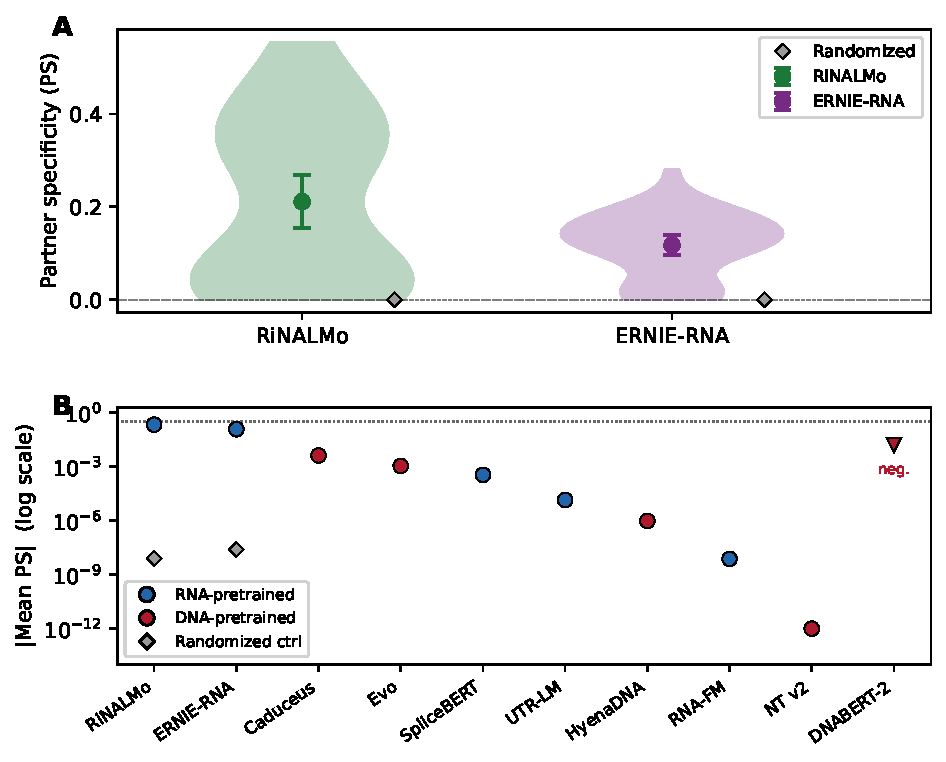
\includegraphics[width=0.85\textwidth]{../figures/figure3_partner_specificity.pdf}
\caption{Partner specificity across ten models. (A)~Per-family PS
distributions for RiNALMo and ERNIE-RNA (violins) with bootstrap 95\%
CIs (error bars); randomized-weight controls (grey diamonds) produce
PS indistinguishable from zero. (B)~$|\text{Mean PS}|$ on log scale
for all ten models, sorted by PS. RiNALMo and ERNIE-RNA exceed the
remaining models by two orders of magnitude. DNABERT-2 (negative PS)
is marked separately.}
\label{fig:ps}
\end{figure}


\subsection{The randomly initialized control}
\label{sec:random-init}

Seven models were also run with every parameter re-initialized, holding the
architecture and the tokenizer and destroying the learned weights. ERNIE-RNA's
control clears each rung of the ladder. At Rung 1 it exceeds its
composition-preserving null in 10 of $\panelN{}$ families against a chance
expectation of 2.4, retains 6 of those at Rung 2, and reaches per-pair precision
$0.490$ at Rung 3 against a chance rate of $0.241$. Judged against the
registered threshold of $1/3$ it passes, at pooled binomial $p = 2.4 \times
10^{-4}$.

The cause is a tensor that randomization does not reach.
\texttt{ErnieRnaModel} holds \texttt{pairwise\_bias\_map}, a
vocabulary-square buffer registered non-persistent, which after the first
forward pass contains six non-zero cells: A--U and U--A at $2.0$, C--G and G--C
at $3.0$, G--U and U--G at $0.8$. Re-initialization iterates a model's
parameters, and a buffer is not a parameter, so the control retains a hardcoded
Watson--Crick and wobble table while its weights are random.

% Written by scripts/generate_ablation_table.py. Do not edit.
\begin{table}[htbp]
\centering
\caption{ERNIE-RNA with and without its pairwise bias buffer, trained and
randomly initialized. Per-pair precision is the fraction of eligible pairs whose
partner is perturbed more than either of its stem neighbours. Chance is the same
fraction under a within-stem derangement, where the assigned partner is false by
construction, and excess is their difference. All four arms cover the same 35
families. Ablation zeroes \texttt{pairwise\_bias\_map} and
\texttt{pairwise\_bias\_proj} and sets the rebuild guard, without which the
first forward pass restores the buffer.}
\label{tab:ablation}
\begin{tabular}{@{}lccc@{}}
\toprule
\textbf{Arm} & \textbf{Precision} & \textbf{Chance} & \textbf{Excess} \\
\midrule
Trained, bias intact         & 0.888 & 0.124 & $+0.764$ \\
Trained, bias ablated        & 0.842 & 0.118 & $+0.725$ \\
Random-init, bias intact     & 0.490 & 0.241 & $+0.249$ \\
Random-init, bias ablated    & 0.267 & 0.255 & $+0.012$ \\
\bottomrule
\end{tabular}
\end{table}


Ablating that table and the projection above it, with the model's rebuild guard
set so the first forward pass cannot restore it, separates the two arms
(Table~\ref{tab:ablation}). Writing excess as precision minus that arm's own
chance rate, the randomly initialized model falls from $+0.249$ to $+0.012$,
while the trained model falls from $+0.764$ to $+0.725$. The difference between
those losses is $+0.198$ (95\% CI $[+0.069, +0.320]$), and the trained model's
remaining excess is $+0.725$ ($[+0.597, +0.836]$), both over
$\chanceRateN{}$ families with $\bootstrapB{}$ resamples. Predictions and
criteria were fixed before either ablated arm was computed.

Across the other nine models no buffer encodes anything about base pairing;
the rest carry position indices, rotary frequencies, or all-zero token-type
vectors, which survive randomization and record where a nucleotide sits. Two
controls nonetheless sat above their own chance rates, RiNALMo by $0.105$ and
RNA-FM by $0.093$. Both excesses come from the layer choice. Per-pair precision
is read at the layer maximizing mean PS within each family, which is
\chanceRateN{} independent selections, and a control with no partner-specific
response collects the maximum of a noise profile in each of them. Choosing one
layer for the whole panel puts RiNALMo at $-0.074$ and RNA-FM at $-0.087$
against their own chance rates and moves the two trained models by at most
$0.010$; choosing the layer on half the families and reporting precision on the
other half reproduces both to three decimals
(Table~\ref{tab:layer-selection}). The same control removes the excess of every
model in the panel except these two and ERNIE-RNA's own bias-carrying control.

\subsection{Multi-sequence replication}
\label{sec:multiseq-results}

Each family is represented in the panel by one curated sequence, so a ratio
could be a property of that sequence rather than of the family. We therefore
score 3--5 members of each family's Rfam seed alignment, \multiseqN{} sequences
over \multiseqFamilies{} families, and measure the within-family coefficient of
variation of the stem--loop ratio. Every model is scored on the same set.

\begin{table}[htbp]
\centering
\caption{Multi-sequence replication. Each family contributes 3--5 members of its Rfam seed alignment, giving 230 sequences over 47 families, and every model is scored on the same set. CV is the within-family coefficient of variation of the stem--loop sensitivity ratio, averaged over families. Three sequences carrying IUPAC ambiguity codes are excluded for every model (\texttt{Corona\_5UTR\_seq0}, \texttt{Corona\_5UTR\_seq1}, \texttt{Corona\_5UTR\_seq3}). A low CV means the ratio is a property of the family rather than of the one curated representative.}
\label{tab:multiseq}
\begin{tabular}{@{}lrrr@{}}
\toprule
\textbf{Model} & \textbf{Mean ratio} & \textbf{Mean CV} & \textbf{Median CV} \\
\midrule
RNA-FM & 1.904 & 0.360 & 0.363 \\
Evo & 1.334 & 0.180 & 0.155 \\
ERNIE-RNA & 1.256 & 0.059 & 0.057 \\
Caduceus & 1.210 & 0.060 & 0.046 \\
HyenaDNA & 1.171 & 0.093 & 0.088 \\
RiNALMo & 1.135 & 0.036 & 0.032 \\
NT~v2 & 1.091 & 0.044 & 0.039 \\
UTR-LM & 1.059 & 0.025 & 0.023 \\
SpliceBERT & 1.049 & 0.027 & 0.023 \\
DNABERT-2 & 0.997 & 0.054 & 0.049 \\
\bottomrule
\end{tabular}
\end{table}


Seven of the ten models vary by under 6\% within a family, from UTR-LM at
$0.025$ to Caduceus at $0.060$ (Table~\ref{tab:multiseq}). For those models the
ratio is a property of the family and the single curated representative is a
fair stand-in for it.

RNA-FM and Evo are the exceptions, at $\cvRNAFM{}$ and $\cvEvo{}$. Both also
fail composition control (Section~\ref{sec:composition-results}): RNA-FM has the
panel's largest raw ratio and exceeds the nucleotide-stratified null in
$\exceedRNAFM{}$ families. A ratio that moves by a third between members of the
same family, and vanishes under a composition null, is what a
sequence-composition response looks like rather than a structural one.

The two models that clear Rung 3 are among the most stable, at $\cvRiNALMo{}$
and $\cvErnieRNA{}$.

\subsection{Robustness analyses}
\label{sec:robustness}

The dinucleotide-stratified null absorbs the sole family (tRNA-Ala)
surviving the nucleotide-stratified null for RNA-FM; second-order sequence
context accounts for the residual signal. Replacing
mean aggregation with median changes PS estimates by $< 5$\% for RiNALMo
and ERNIE-RNA and does not alter the model ranking. Reading PS at the last
layer rather than each family's best changes RiNALMo by $-0.1$\% and ERNIE-RNA
by $-1.9$\%, because both peak at or beside their final layer
(Section~\ref{sec:ps-results}). Restricting to Watson--Crick pairs only (excluding wobble G--U
pairs) does not change the primary conclusions. Widening the PS neighbor
window from $\pm 1$ to $\pm 2$ positions reduces PS magnitudes uniformly
across models without altering their relative ranking.
A transversion control (\transversionAlphabet{}, substitutions that disrupt
pairing without being complement swaps) reproduces the Watson--Crick ratios
across all ten models, with the widest deviation \transversionWidestDeviation{}
at \transversionWidest{} and seven models inside $2.2$\%
(Table~\ref{tab:transversion}). The stem--loop contrast is not an artifact of
the substitution alphabet. Five of the seven randomized-weight
controls produce $|\text{mean PS}| < 10^{-8}$. The two that do not are the
multi-nucleotide tokenizers, NT~v2 at $-3.4 \times 10^{-5}$ and DNABERT-2 at
$-4.0 \times 10^{-4}$, the second comparable in magnitude to its trained value.
The two Rung 3 statistics disagree on these controls: ERNIE-RNA's has mean PS
$3.4 \times 10^{-9}$ and per-pair precision $0.490$, so a mean PS at zero does
not place a control at chance.

The attention--contact channel, the transversion control, the registered
hypotheses and the run provenance appear in Appendix~\ref{app:supplement};
per-family ratios, gate outcomes and partner specificity are in Supplementary
Tables~S2 and~S3.


Twenty-one hypotheses registered across four protocols, each hashed before its
data were collected, produce nine confirmations and eleven failures
(Table~\ref{tab:hypotheses}). The registered prediction that RNA-pretrained
models would outperform DNA-pretrained models on partner specificity failed
($r_b = \domainRankBiserial{}$, $p = \domainP{}$): Caduceus (7.7M, DNA) exceeds
three RNA models on mean PS.


\subsection{Covariation versus geometry}
\label{sec:covariation-results}

Partner specificity could reflect sequence covariation rather than
learned geometric pairing. Compensatory mutations that maintain base
pairing are overrepresented in evolutionary RNA alignments; a model
trained on such sequences might predict that mutating one position
perturbs its covarying partner without encoding the physical mechanism
of pairing.

To test this, each panel family was regenerated \synPerFamily{} times with its
dot-bracket structure preserved exactly and its nucleotides reassigned---uniform
Watson--Crick pairs at paired positions, uniform elsewhere---giving \synN{}
sequences that share structure with their natural counterparts and carry no
evolutionary covariation. All ten models were run on them
(Table~\ref{tab:synthetic}).

\begin{table}[htbp]
\centering
\caption{Partner specificity on natural and synthetic sequences. Synthetic sequences keep each family's dot-bracket structure and reassign its nucleotides -- uniform Watson--Crick pairs at paired positions, uniform elsewhere -- five per family, so they carry no evolutionary covariation. Excess is per-pair precision minus that arm's own within-stem derangement chance rate, over 35 natural and 195 synthetic sequences. Mean PS falls further than excess precision does, because PS is a magnitude and the synthetic sequences are less structured in composition.}
\label{tab:synthetic}
\small
\begin{tabular}{@{}lrrrrr@{}}
\toprule
 & \multicolumn{2}{c}{\textbf{Mean PS}} & \multicolumn{3}{c}{\textbf{Excess precision over own chance}} \\
\cmidrule(lr){2-3}\cmidrule(lr){4-6}
\textbf{Model} & \textbf{Natural} & \textbf{Synthetic} & \textbf{Natural} & \textbf{Synthetic} & \textbf{Retained} \\
\midrule
RiNALMo (650M) & 0.2062 & 0.0919 & +0.770 & +0.582 & 76\% \\
ERNIE-RNA (86M) & 0.1113 & 0.0415 & +0.764 & +0.574 & 75\% \\
Caduceus (14M) & 0.0039 & 0.0036 & +0.122 & +0.058 & 48\% \\
Evo (7B) & 0.0017 & 0.0013 & +0.040 & +0.016 & --- \\
HyenaDNA (5.4M) & $2.4 \times 10^{-4}$ & $1.5 \times 10^{-4}$ & -0.010 & +0.005 & --- \\
SpliceBERT (19M) & $2.2 \times 10^{-4}$ & $2.3 \times 10^{-4}$ & +0.009 & +0.057 & --- \\
RNA-FM (99M) & $8.4 \times 10^{-5}$ & $1.4 \times 10^{-4}$ & +0.109 & +0.092 & 85\% \\
UTR-LM ($\sim$2M) & $8.3 \times 10^{-6}$ & $1.5 \times 10^{-5}$ & +0.016 & +0.035 & --- \\
NT~v2 (56M) & $-9.7 \times 10^{-5}$ & $-2.1 \times 10^{-4}$ & +0.000 & -0.001 & --- \\
DNABERT-2 (117M) & -0.0160 & -0.0204 & +0.000 & +0.000 & --- \\
\bottomrule
\end{tabular}
\end{table}


Mean PS falls by \synPSDropErnieRNA{} for ERNIE-RNA, to \synPSErnieRNA{}, and
by \synPSDropRiNALMo{} for RiNALMo, to \synPSRiNALMo{}. Per-pair precision
measured against each arm's own chance rate falls by a quarter: ERNIE-RNA's
excess goes from \natExcessErnieRNA{} to \synExcessErnieRNA{} and RiNALMo's
from \natExcessRiNALMo{} to \synExcessRiNALMo{}, retaining
\synRetainedErnieRNA{} and \synRetainedRiNALMo{}. The two statistics answer
different questions on these sequences. Mean PS is a magnitude, and synthetic
sequences have flatter composition, so every perturbation is smaller. Per-pair
precision asks whether a mutated position's partner moves more than that
partner's neighbors, which is what Rung 3 tests, and three quarters of it
survives on sequences with no covariation at all. Those sequences also destroy
natural sequence context, so the quarter that is lost is an upper bound on the
covariation contribution and the three quarters that remain are a lower bound
on the rest.

As an independent check, we computed mutual information (MI) between
paired positions from the Rfam seed alignments of the \panelN{} panel families.
MI separates paired from unpaired positions (mean MI $= 0.347$ against
$0.066$; Wilcoxon $p = 7.1 \times 10^{-14}$), confirming that evolutionary
covariation is detectable in the alignments. Per-family mean MI does not
correlate significantly with model PS (RiNALMo: $\rho = +0.272$, $p = 0.109$;
ERNIE-RNA: $\rho = +0.239$, $p = 0.160$; $n = \confirmatoryN{}$). Families with strong covariation signal
do not systematically produce higher PS, suggesting that the models'
partner specificity reflects learned structure rather than
recapitulated covariation.


\subsection{HTT case study}
\label{sec:htt-results}

The CAG repeat region in huntingtin exon~1 forms hairpin structures whose
stability scales with repeat count \citep{demezer2011mutant,
krzyzosiak2012triplet}. We evaluated five HTT exon~1 fragments
(NM\_002111.7) with CAG repeat counts of 17, 21, 36, 40 and 60, folded with
ViennaRNA RNAfold \citep{lorenz2011viennarna}, through the panel's own stages.

\begin{table}[htbp]
\centering
\caption{Five HTT exon~1 fragments with CAG repeat counts 17, 21, 36, 40 and 60, folded with ViennaRNA. Ratio and $>$~null are stem--loop mutation sensitivity against the nucleotide-stratified null; Attn~$\rho$ is the mean Spearman correlation between self-attention and the contact map, absent for the state-space models; Probing is linear-probe accuracy for stem-versus-loop classification. CAG60 is cosine distance from the CAG17 fragment, at the final layer and at the embedding layer. The repeat region contains no U, so a linear probe has an extreme composition bias available to it, and the fragments differ in length, so embedding distance rises with repeat count at the embedding layer for every model ($\rho = +1.00$) before any block has run.}
\label{tab:htt}
\small
\begin{tabular}{@{}lrcrrrr@{}}
\toprule
\textbf{Model} & \textbf{Ratio} & \textbf{$>$ null} & \textbf{Attn $\rho$} & \textbf{Probing} & \textbf{CAG60 last} & \textbf{CAG60 best} \\
\midrule
RiNALMo & 1.031 & 0/5 & 0.054 & 0.983 & 0.0679 & 0.0115 \\
ERNIE-RNA & 1.086 & 0/5 & 0.070 & 0.985 & 0.0229 & 0.2130 \\
RNA-FM & 1.800 & 1/5 & 0.036 & 0.792 & $2.2 \times 10^{-7}$ & 0.0151 \\
UTR-LM & 1.151 & 1/5 & 0.039 & 0.971 & 0.0158 & 0.0134 \\
SpliceBERT & 0.996 & 0/5 & 0.036 & 0.975 & 0.0424 & 0.2120 \\
Caduceus & 1.231 & 0/5 & --- & 0.977 & 0.0017 & 0.0070 \\
HyenaDNA & 1.045 & 0/5 & --- & 0.926 & 0.0193 & 0.0249 \\
NT~v2 & 1.012 & 0/5 & 0.124 & 0.623 & 0.0120 & 0.1509 \\
DNABERT-2 & 0.998 & 0/5 & 0.140 & 0.612 & 0.5073 & 0.5073 \\
\bottomrule
\end{tabular}
\end{table}


\httHighProbing{} of \httModels{} models reach linear-probe accuracy above
$0.97$ for stem-versus-loop classification, and \httHighProbingClean{} of those
exceed the composition-preserving null in no more than one of the five
fragments. The repeat region contains only C, A and G---no U---so a linear
probe has an extreme composition bias available to it.

Embedding distance from the CAG17 fragment rises monotonically with repeat
count for all \httMonotone{} models with more than one layer, at Spearman
$\rho = +1.00$, and does so at the embedding layer before any block has run:
the fragments have lengths 235 to 364 and differ in composition accordingly.
The measure separates the fragments by construction and does not rank models by
whether they represent the expansion. RNA-FM is the one model whose final layer
departs from the pattern, its distances there collapsing to
$2 \times 10^{-7}$ in float64.

High probing accuracy on a computationally predicted structure coexists with
null composition-controlled signal: apparent structure decoding persists in a
strongly composition-biased context.


% ============================================================================
% DISCUSSION — 7 paragraphs
% ============================================================================
\section{Discussion}
\label{sec:discussion}

% P1: Primary conclusion + positive result
Composition-matched nulls absorb most of the apparent stem--loop
sensitivity across all ten models. Two RNA-pretrained models---RiNALMo and
ERNIE-RNA---retain reproducible partner-specific responses under the most
stringent test. Multi-sequence replication shows low within-family
variance across eight of ten models.

% P2: Why composition matching changes interpretation
The underlying problem is general: whenever a structural annotation
correlates with feature composition, any embedding metric sensitive to
feature identity inherits the correlation. The nucleotide-stratified
permutation null controls for this by breaking the structure--composition
link while preserving nucleotide identity. The same template applies to
any biological structure correlated with sequence composition.

% P3: Interpret positive models cautiously
RiNALMo and ERNIE-RNA reach partner specificity through different pathways.
ERNIE-RNA injects a base-pairing attention bias, and that bias with random
weights above it resolves partners at $0.490$ against a chance rate of $0.241$;
ablating it removes the control's excess and costs the trained model $0.039$.
RiNALMo uses standard attention with no structural bias and reaches comparable
precision at $\paramsOverRiNALMo{}\times$ the parameters. On synthetic sequences that preserve
structure and destroy covariation (Section~\ref{sec:covariation-results}), both
retain roughly three quarters of their excess over chance. Those sequences also
destroy natural sequence context, so the quarter that is lost bounds the
covariation contribution from above and the three quarters that remain bound
the non-covariation contribution from below. Whether that remainder reflects a
geometric internal model of folding or a statistical regularity of paired
positions is open.

% P4: What predicts composition-controlled sensitivity
Neither training domain nor architecture family alone predicts
composition-controlled sensitivity. The three state-space models span mean
ratios $\ratioHyenaDNA{}$ to $\ratioEvo{}$ and the seven transformers
$\ratioDNABERTTwo{}$ to $\ratioRNAFM{}$, so the architecture families overlap
almost entirely. Evo at $\ratioEvo{}$ exceeds four of the five RNA-pretrained
models on the raw ratio and Caduceus at $\ratioCaduceus{}$ exceeds three. The two models
that survive the partner specificity test (RiNALMo and ERNIE-RNA) share
RNA pretraining but differ in mechanism: ERNIE-RNA injects explicit
base-pairing attention bias, while RiNALMo uses standard self-attention at
$\paramsOverRiNALMo{}\times$ the parameters. Scale alone does not explain the result:
Evo at 7B parameters produces high raw ratios but high within-family
variance, and its signal is largely absorbed by composition nulls. What
distinguishes the two positive models from the remaining eight is an open
question whose answer likely requires internal mechanistic analysis rather
than further behavioral benchmarking.

% P5: Broader evaluation implications
RNA structure prediction benchmarks have moved toward stricter evaluation
because high apparent performance can fail to generalize across families
\citep{szikszai2022generalization}. This work extends the concern from
dataset similarity to sequence-composition confounding. NT~v2 and DNABERT-2
show near-zero embedding-level partner specificity while passing many families
at the composition gate, and their attention--contact correlations do not
supply the missing channel: NT~v2 reads $\attnNTvTwo{}$ trained against
$\attnUntrainedNTvTwo{}$ randomly initialized, so its correlation is
architectural, and DNABERT-2's trained excess of $\attnDeltaDNABERTTwo{}$ rests
on a model that does not reproduce itself between runs
(Table~\ref{tab:attn_trained_untrained}).

% P6: Limitations
% (Updated to reference covariation results in Section 2.5)
\paragraph{Limitations.}
The complement-swap metric tests sensitivity to single base-pair disruptions;
it does not test tertiary contacts, pseudoknots, or long-range interactions.
The synthetic covariation control (Section~\ref{sec:covariation-results})
removes covariation and natural sequence context together, so the quarter of
the excess it costs is an upper bound on what covariation contributes. HTT structures
are RNAfold predictions. Ten models do not cover the full model space. Pretraining-set contamination cannot be
fully reconstructed. Multi-nucleotide tokenization limits direct
comparability for NT~v2 and DNABERT-2.

\paragraph{Practical recommendations.}
Any claim that an RNA representation encodes secondary structure should
report stem--loop sensitivity alongside a nucleotide-stratified null, so
readers can separate composition sensitivity from structure awareness.
Partner specificity is more informative than aggregate stem--loop contrasts:
a model that perturbs stems more than loops may respond to GC content, while
one that selectively perturbs the annotated pairing partner encodes
positional pairing information. Randomized-weight controls should establish
each architecture's baseline capacity. Replication across
multiple sequences per family guards against single-sequence artifacts; a
coefficient of variation above 10\% signals instability. For
multi-nucleotide tokenizers, the mapping from token-level to position-level
metrics should be stated explicitly.


% ============================================================================
% MATERIALS AND METHODS (after Discussion per RNA journal format)
% ============================================================================
\section{Materials and Methods}
\label{sec:methods}

\subsection{Benchmark construction}
\label{sec:benchmark}

We evaluate \panelN{} Rfam~14.10 families \citep{kalvari2021rfam} spanning ribozymes, riboswitches, snRNAs,
cis-regulatory elements, miRNA precursors, CRISPR repeats, and other ncRNAs.
Positions are labeled stem or loop from consensus dot-bracket annotation.
Minimum inclusion criteria: $\geq 20$~nt, $\geq 5$ stem and $\geq 5$ loop
positions. Pseudoknots, noncanonical pairs, and gap positions are excluded.

All structures are consensus secondary structures from Rfam seed alignments;
none are experimentally determined crystal or cryo-EM structures. Pretraining
data overlap cannot be fully reconstructed for all models. The full family
list with accessions appears in Table~\ref{tab:panel}.

\subsection{Models and controls}
\label{sec:models}

\begin{table}[htbp]
\centering
\caption{Models evaluated.}
\label{tab:models}
\begin{tabular}{@{}llrll@{}}
\toprule
\textbf{Model} & \textbf{Domain} & \textbf{Params} & \textbf{Architecture} & \textbf{Tokenization} \\
\midrule
RNA-FM \citep{rnafm}                    & RNA & 99M  & Transformer           & Character \\
RiNALMo \citep{rinalmo}                 & RNA & 650M & Transformer           & Character \\
ERNIE-RNA \citep{yin2024ernierna}        & RNA & 86M  & Transformer$^\dagger$ & Character \\
SpliceBERT \citep{chen2024splicebert}     & RNA & 19M  & Transformer           & Character \\
UTR-LM \citep{chu2024utrlm}             & RNA & 1.2M & Transformer           & Character \\
NT~v2 \citep{dalla2023nucleotide}        & DNA & 56M  & Transformer           & 6-mer     \\
DNABERT-2 \citep{zhou2024dnabert2}       & DNA & 117M & Transformer           & BPE       \\
Caduceus \citep{schiff2024caduceus}      & DNA & 7.7M & Mamba (SSM)           & Character \\
HyenaDNA \citep{nguyen2024hyenadna}      & DNA & 0.45M & Hyena (SSM)          & Character \\
Evo \citep{nguyen2024evo}                & DNA & 7B   & StripedHyena          & Character \\
\bottomrule
\end{tabular}
\medskip

\small $^\dagger$ERNIE-RNA injects a base-pairing attention bias from the
second layer onward.
\end{table}

We evaluate ten models covering attention, SSM, and hybrid architectures
(Table~\ref{tab:models}): five pretrained on RNA, five on DNA.
Randomized-weight controls for all ten models reinitialize all
learned parameters (Xavier normal for matrices, $\mathcal{N}(0, 0.02)$
for vectors) while preserving architecture. NT~v2 and DNABERT-2 use
multi-nucleotide tokenization (6-mer and BPE), limiting direct
comparability for position-level metrics.

\subsection{Perturbation tests}
\label{sec:perturbation}

For each annotated position, we swap the nucleotide with its Watson--Crick
complement (A$\leftrightarrow$U, C$\leftrightarrow$G) and measure the cosine
distance between wild-type and mutant embeddings at that position, maximized
over layers. Cosine distance is scale-invariant across architectures.
For multi-nucleotide tokenization, token-level outputs are mapped to
nucleotide positions by distributing the token embedding equally across
constituent nucleotides.

\paragraph{Nucleotide-stratified null.}
Stem/loop labels are shuffled within each nucleotide type (1{,}000
permutations), preserving nucleotide identity while breaking its structural
label. Layer selection is repeated inside every permutation. A
dinucleotide-stratified extension additionally conditions on the 3' neighbor.

\paragraph{Partner specificity.}
\label{sec:ps-method}
For each Watson--Crick pair $(i, j)$ where $j$ is the annotated partner:
\[
\text{PS}(i,j) = \Delta_j - \max(\Delta_{j-1}, \Delta_{j+1})
\]
where $\Delta_k$ is the cosine distance at position $k$ after the complement
swap at position $i$. Positive PS indicates the model perturbs the true
partner more than its immediate neighbors. Chance for the per-pair comparison
is measured rather than assumed: partner assignments are permuted within each
stem under a derangement (500 derangements), so every position keeps its stem,
its nucleotide and its layer while its assigned partner is false by
construction. Measured this way the chance rate ranges from $0.000$ to $0.316$
across the panel.

\paragraph{Covariation control.}
To distinguish learned geometric sensitivity from recapitulated evolutionary
covariation, synthetic sequences were generated for each family: dot-bracket
structure preserved exactly, nucleotides assigned randomly (uniform
Watson--Crick pairs at paired positions, uniform random at unpaired). Mutual
information (MI) between paired and unpaired positions was computed from Rfam
seed alignments as an independent covariation measure.

\subsection{Statistical analysis and replication}
\label{sec:stats}

The biological unit of replication is the RNA family. The primary outcome is
partner specificity (PS); the primary comparison is trained vs.\
randomized-weight PS. A family is \emph{gate-qualifying} for a given model
if its raw stem--loop sensitivity ratio exceeds the nucleotide-stratified
null at the 95th percentile. PS is computed only over gate-qualifying
families and aggregated as their mean.

To test stability across biological replicates, the Rung~1 stage is repeated on
the seed-alignment members of each panel family: \multiseqN{} sequences across
\multiseqFamilies{} families, 3--5 per family, each scored as its own family and
regrouped afterwards. Within-family coefficient of variation (CV) quantifies
replication stability. Three sequences carrying IUPAC ambiguity codes outside
\texttt{ACGTUN} are excluded for every model, so the comparison is over a common
set.

Family-level bootstrap resampling (10{,}000 iterations, seed 42)
provides 95\% CIs for mean PS and mean sensitivity ratio. For the binary
gate test, each family's ratio is compared to its own 95th-percentile
permutation null; we report the count exceeding this threshold alongside
the expected false-positive count under independence
($m \times \alpha = \panelN{} \times 0.05 = \expectedFalsePositives{}$).
Bonferroni correction
($\alpha / m \approx 0.001$) provides a conservative bound.


% ============================================================================
% DATA AVAILABILITY
% ============================================================================
\section*{Data and Code Availability}

All data, scripts, and pre-registration protocols are available at
\url{https://github.com/elliottower/rna-structure-audit} and archived at
Zenodo (DOI: \href{https://doi.org/10.5281/zenodo.21362717}{10.5281/zenodo.21362717}).

The deposited panel holds one directory per model, each stamped with the commit
and library versions it was computed under. Preregistrations are frozen at a
commit hash, deviations are dated in \texttt{DEVIATIONS.md}, and reported numbers
are bound to their runs, using \texttt{prereg}, \texttt{results} and
\texttt{citations} \citep{tower2026reproducible}.


% ============================================================================
% DECLARATIONS
% ============================================================================
\section*{Acknowledgements}

The author used Claude Code \citep{anthropic2025claude} to assist with
drafting manuscript text and with writing and debugging analysis code.
The author reviewed and verified all outputs, takes full responsibility
for the accuracy and integrity of the work, and confirms that all
hypotheses, preregistered predictions, interpretations, and conclusions
are the author's own.

\paragraph{Ethics approval and consent to participate.}
This study uses exclusively publicly available pretrained model weights
and published RNA sequences. No human subjects or animal subjects were
involved. No ethical approval was required.

\paragraph{Competing interests.} The author declares no competing interests.

\paragraph{Funding.} None. This work was conducted independently.

\paragraph{Author contributions.} E.T.: Conceptualization, Methodology,
Software, Formal analysis, Investigation, Data curation, Writing ---
original draft, Writing --- review \& editing, Visualization.


% ============================================================================
% REFERENCES
% ============================================================================
\appendix
\section{Supplementary tables}
\label{app:supplement}

% Generated by scripts/generate_panel_description.py. Do not edit.
\begin{longtable}{llllrp{0.28\textwidth}}
\caption{The curated panel. Families above the rule are analyzed; those below carry an annotation that could not be repaired against the Rfam seed alignment and are withdrawn. Accession names the seed member a record's sequence and structure come from.}\\
\toprule
\textbf{Family} & \textbf{Class} & \textbf{Rfam} & \textbf{Accession} & \textbf{nt} & \textbf{Note} \\
\midrule\endfirsthead
\toprule
\textbf{Family} & \textbf{Class} & \textbf{Rfam} & \textbf{Accession} & \textbf{nt} & \textbf{Note} \\
\midrule\endhead
6S\_RNA & other ncRNAs & RF00013 & M12965.1/109-292 & 184 &  \\
7SK\_RNA & other ncRNAs & RF00100 & AAGU03002674.1/25068-24736 & 333 &  \\
Bacterial\_SRP & other ncRNAs & RF00169 & AE016826.1/499549-499447 & 103 &  \\
CRISPR\_leader & CRISPR repeats & RF01315 & CP000679.1/62025-62054 & 30 &  \\
Corona\_5UTR & cis-regulatory elements & RF03120 & MT019530.1/1-299 & 299 &  \\
Corona\_s2m & cis-regulatory elements & RF00164 & Z66541.1/2326-2368 & 43 &  \\
CrPV\_IRES & cis-regulatory elements & RF00458 & AF218039.1/6028-6223 & 196 &  \\
FMN\_riboswitch & riboswitches & RF00050 & AE017263.1/670666-670782 & 117 &  \\
HDV\_ribozyme & ribozymes & RF00094 & AF209859.1/689-775 & 87 & record repaired \\
Hepatitis\_C\_IRES\_III & cis-regulatory elements & RF00061 & AB047639.1/2-353 & 352 &  \\
Histone\_3prime & cis-regulatory elements & RF00032 & CAAE01014536.1/93243-93288 & 46 &  \\
IRE\_stem\_loop & cis-regulatory elements & RF00037 & BC063337.1/26-62 & 37 &  \\
SAH\_riboswitch & riboswitches & RF01057 & CP000744.1/550599-550494 & 106 &  \\
SAM\_riboswitch & riboswitches & RF00162 & URS000080DDBE\_1423/1-119 & 119 & structure repaired \\
SECIS\_element & cis-regulatory elements & RF00031 & AF288740.1/1291-1357 & 67 &  \\
THF\_riboswitch & riboswitches & RF01831 & AAXG02000014.1/43071-43187 & 117 &  \\
TPP\_riboswitch & riboswitches & RF00059 & AARF01000324.1/6363-6261 & 103 & record repaired \\
T\_box\_leader & cis-regulatory elements & RF00230 & AE005176.1/68627-68394 & 234 &  \\
U1\_snRNA & snRNAs & RF00003 & M32270.1/371-535 & 165 &  \\
U4\_snRNA & snRNAs & RF00015 & AM479189.1/4511-4661 & 151 &  \\
U5\_snRNA & snRNAs & RF00020 & AAZX01000523.1/17560-17680 & 121 &  \\
U6\_snRNA & snRNAs & RF00026 & AFQF01002057.1/12805-12639 & 167 &  \\
Vault\_RNA & other ncRNAs & RF00006 & AAHX01094554.1/16303-16446 & 144 &  \\
Y\_RNA & other ncRNAs & RF00019 & ABDC01154708.1/21315-21214 & 102 &  \\
ZMP\_riboswitch & riboswitches & RF01750 & CU914168.1/2467319-2467448 & 130 &  \\
c\_di\_GMP\_riboswitch & riboswitches & RF01051 & CP001098.1/769828-769735 & 94 &  \\
cobalamin\_riboswitch & riboswitches & RF00174 & CP000830.1/164274-164053 & 222 &  \\
fluoride\_riboswitch & riboswitches & RF01734 & CP000240.1/171311-171206 & 106 &  \\
glmS\_ribozyme & ribozymes & RF00234 & FJ935779.1/2022-2192 & 171 &  \\
glycine\_riboswitch & riboswitches & RF00504 & AE008691.1/313165-313055 & 111 &  \\
group\_II\_intron\_D5 & other ncRNAs & RF00029 & Z00044.2/12705-12618 & 88 &  \\
group\_I\_intron\_P4P6 & other ncRNAs & RF00028 & M86534.1/28-414 & 387 &  \\
hammerhead\_ribozyme & ribozymes & RF00163 & AF036748.1/120-164 & 45 & record repaired \\
hatchet\_ribozyme & ribozymes & RF02678 & URS0000D6BD63\_12908/19-166 & 148 &  \\
lysine\_riboswitch & riboswitches & RF00168 & M93419.1/332-511 & 180 &  \\
manganese\_riboswitch & riboswitches & RF01786 & AACY020292692.1/343-428 & 86 &  \\
mir\_122\_precursor & miRNA precursors & RF00684 & URS00000BAFD3\_9823/7-79 & 73 &  \\
mir\_155\_precursor & miRNA precursors & RF00731 & URS000062749E\_9606/1-65 & 65 &  \\
mir\_21\_precursor & miRNA precursors & RF00658 & URS0000013967\_10029/11-82 & 72 &  \\
mir\_let7\_precursor & miRNA precursors & RF00027 & AAIY01003579.1/1841-1762 & 80 &  \\
pistol\_ribozyme & ribozymes & RF02679 & AGFS01138167.1/426-348 & 79 &  \\
preQ1\_riboswitch & riboswitches & RF00522 & AE004439.1/209165-209100 & 66 &  \\
purine\_riboswitch & riboswitches & RF00167 & BA000043.1/272473-272574 & 102 &  \\
tRNA\_Ala\_human & tRNAs & RF00005 & --- & 75 &  \\
tRNA\_Phe\_yeast & tRNAs & RF00005 & --- & 76 &  \\
tmRNA & other ncRNAs & RF00023 & CP000033.3/728512-728880 & 369 &  \\
twister\_ribozyme & ribozymes & RF02681 & URS0000D6974B\_12908/1-116 & 116 &  \\
\midrule
5S\_rRNA\_ecoli & rRNAs & RF00001 & --- & 120 & withdrawn: the name asserts E. coli; RF00001's seed carries no E. coli member; a substitute would leave the name false, and the stored sequence needs an annotation from outside the seed alignment \\
IRES\_HCV\_domainII & cis-regulatory elements & --- & --- & 86 & withdrawn: the name asserts domain II of the HCV IRES, not the whole IRES; every seed member is a whole molecule \\
RNaseP\_specificity & other ncRNAs & RF00010 & --- & 94 & withdrawn: the name asserts the specificity domain of RNase P, not the whole RNA; every seed member is a whole molecule \\
SRP\_RNA\_helix8 & other ncRNAs & RF00017 & --- & 90 & withdrawn: no RF00017 member projects to a structure under 5\% non-canonical \\
U2\_snRNA\_stem & snRNAs & RF00004 & --- & 83 & withdrawn: the name asserts a stem of U2 snRNA, not the whole snRNA; every seed member is a whole molecule \\
\bottomrule
\end{longtable}


\begin{table}[htbp]
\centering
\caption{Attention-contact Spearman correlation, trained against randomly
initialized weights, for the seven models in the panel that expose attention.
$\Delta$ within $\pm 0.05$ is read as architectural: the
correlation is present before any pretraining. Both columns are means over the
repaired panel, computed with eager attention.}
\label{tab:attn_trained_untrained}
\small
\begin{tabular}{@{}lccl@{}}
\toprule
\textbf{Model} & \textbf{Trained} & \textbf{Untrained} & \textbf{Interpretation} \\
\midrule
NT~v2        & 0.234 & 0.241 & Architectural ($\Delta = -0.007$) \\
DNABERT-2    & 0.196 & 0.153 & Architectural ($\Delta = +0.043$) \\
ERNIE-RNA    & 0.113 & 0.085 & Architectural ($\Delta = +0.027$) \\
RiNALMo      & 0.107 & 0.064 & Architectural ($\Delta = +0.044$) \\
SpliceBERT   & 0.054 & 0.032 & Architectural ($\Delta = +0.022$) \\
UTR-LM       & 0.051 & 0.054 & Architectural ($\Delta = -0.003$) \\
RNA-FM       & 0.048 & 0.043 & Architectural ($\Delta = +0.005$) \\
\bottomrule
\end{tabular}
\end{table}


\begin{table}[htbp]
\centering
\caption{Mutation sensitivity under the Watson-Crick substitution and under a
substitution that leaves no position paired with the partner it had (A$\to$C, C$\to$A, G$\to$U, U$\to$C; T
follows U). Rows are ordered by the size of the change. A model whose ratio
depends on the substituted nucleotide being a complement rather than on the
pairing being broken would move between the two columns.}
\label{tab:transversion}
\small
\begin{tabular}{lrrr}
\toprule
\textbf{Model} & \textbf{Watson-Crick} & \textbf{Transversion} & \textbf{Change} \\
\midrule
HyenaDNA (5.4M, DNA)       & 1.160 & 1.073 & $-7.5$\% \\
Caduceus (14M, DNA)        & 1.206 & 1.158 & $-4.0$\% \\
ERNIE-RNA (86M, RNA)       & 1.276 & 1.253 & $-1.7$\% \\
DNABERT-2 (117M, DNA)      & 1.003 & 0.988 & $-1.5$\% \\
RNA-FM (99M, RNA)          & 1.722 & 1.701 & $-1.2$\% \\
NT~v2 (56M, DNA)           & 1.113 & 1.124 & $+1.0$\% \\
SpliceBERT (19M, RNA)      & 1.040 & 1.051 & $+1.0$\% \\
Evo (7B, DNA)              & 1.450 & 1.465 & $+1.0$\% \\
UTR-LM ($\sim$2M, RNA)     & 1.056 & 1.058 & $+0.2$\% \\
RiNALMo (650M, RNA)        & 1.143 & 1.144 & $+0.1$\% \\
\bottomrule
\end{tabular}
\end{table}


\begin{table}[htbp]
\centering
\caption{Every registered hypothesis, with the panel it is decided on. Rungs~1
and~2 are decided on the repaired panel of \panelN{} families; Rung~3 on the
36 confirmatory families that qualify after quarantine.
H1 is Phase~1's underpowered form of H6 and is reported at the twelve-family
value it was decided on, because five of the twelve records are withdrawn and
the panel it names no longer exists. H1$_6$ is a single decision requiring both
a positive mean PS by Wilcoxon signed-rank ($p < 0.0167$) and the count
criterion; the count criterion was registered as 7 at $N = 32$ and is
8 at the repaired $N$, and both are
reported in the text. Sources: \texttt{PREREGISTRATION\_EXPANDED\_RFAM}
(H1, H6, H6b, H7, H8, H10, H11), \texttt{PREREG\_PHASE3\_RNA\_PRETRAINED}
(H12--H15), \texttt{PREREG\_PHASE4\_EXPANDED\_MODELS} (H16--H21),
\texttt{PREREGISTRATION\_PHASE6\_V2} (H1$_6$--H3$_6$).}
\label{tab:hypotheses}
\small
\begin{tabular}{lllll}
\toprule
\textbf{Hyp.} & \textbf{Criterion} & \textbf{Panel} & \textbf{Result} & \textbf{Verdict} \\
\midrule
H1       & RNA-FM trained/untrained ratio $\geq 2.0$ & Phase 1, $N = 12$ & 1.74$\times$ & FAIL \\
H6       & RNA-FM trained/untrained ratio $\geq$ 2.0 & repaired, $N = \panelN{}$ & 0.93$\times$ & FAIL \\
H14      & RiNALMo trained/untrained ratio $\geq$ 2.0 & repaired, $N = \panelN{}$ & 0.50$\times$ & FAIL \\
H19      & SpliceBERT trained/untrained ratio $<$ 2.0 & repaired, $N = \panelN{}$ & 0.87$\times$ & \textbf{PASS} \\
H6b      & RNA-FM exceeds nuc.\ null in $\geq \lceil 0.17 N \rceil$ $= 8$ families & repaired, $N = \panelN{}$ & 0/47 & FAIL \\
H7       & $\geq 1$ family survives the dinuc.\ null & repaired, $N = \panelN{}$ & 30 fam (ERNIE-RNA) & \textbf{PASS} \\
H8       & best probing accuracy $>$ 0.5 by $\geq 0.02$ & repaired, $N = \panelN{}$ & 0.683 (ERNIE-RNA) & \textbf{PASS} \\
H10      & RNA-FM trained $>$ untrained in $\geq 75\%$ of families & repaired, $N = \panelN{}$ & 17/47 = 36\% & FAIL \\
H15      & RiNALMo trained $>$ untrained in $\geq 75\%$ of families & repaired, $N = \panelN{}$ & 0/47 = 0\% & FAIL \\
H17      & ERNIE-RNA trained $>$ untrained in $\geq 75\%$ of families & repaired, $N = \panelN{}$ & 7/47 = 15\% & FAIL \\
H11      & NT~v2 attn.\ $> 0.15$ trained and $< 0.05$ untrained & repaired, $N = \panelN{}$ & 0.242 / 0.246 & FAIL \\
H12      & RiNALMo attn.\ $\rho$ $<$ 0.10 & repaired, $N = \panelN{}$ & 0.107 & FAIL \\
H13      & UTR-LM attn.\ $\rho$ $>$ 0.15 & repaired, $N = \panelN{}$ & 0.051 & FAIL \\
H16      & ERNIE-RNA attn.\ $\rho$ $<$ 0.10 & repaired, $N = \panelN{}$ & 0.113 & FAIL \\
H18      & SpliceBERT attn.\ $\rho$ $<$ 0.10 & repaired, $N = \panelN{}$ & 0.054 & \textbf{PASS} \\
H21      & DNABERT-2 attn.\ $\rho$ $<$ 0.20 & repaired, $N = \panelN{}$ & 0.199 & \textbf{PASS} \\
H20      & $|$DNABERT-2 trained $-$ untrained attn.$| < 0.05$ & repaired, $N = \panelN{}$ & 0.009 & \textbf{PASS} \\
H1$_6$   & $\geq 1$ model: PS $> 0$, $\geq 8$ fam $>$ null & confirmatory, $N = 36$ & RiNALMo: 31/32; ERNIE-RNA: 32/34 & \textbf{PASS} \\
H2$_6$   & RNA PS $>$ DNA PS (rb $> 0.5$) & confirmatory, $N = 36$ & rb $= +0.04$, $p = 1.000$ & FAIL \\
H3$_6$   & partner-is-max $> 1/3$ & confirmatory, $N = 36$ & RiNALMo: 0.886; ERNIE-RNA: 0.885 & \textbf{PASS} \\
\bottomrule
\end{tabular}
\end{table}


% Written by scripts/generate_results_tables.py. Do not edit.
\begin{table}[htbp]
\centering
\small
\caption{Provenance for each run behind the results tables. Every run analyzes the same panel (SHA-256 \texttt{5c4d6f6d4c32}, 47 families, 5 withdrawn) under the same family-derived seeding. No single library stack loads all ten models, so the stack is given per run, and so is the commit.}
\label{tab:provenance}
\begin{tabular}{lllll}
\toprule
Model & Weights & Device & Commit & Library stack \\
\midrule
ERNIE-RNA & pretrained & cuda & \texttt{1350db1} & \footnotesize torch 2.6.0, transformers 5.14.1, multimolecule 0.2.0 \\
ERNIE-RNA (untrained) & randomized & cuda & \texttt{1350db1} & \footnotesize torch 2.6.0, transformers 5.14.1, multimolecule 0.2.0 \\
RiNALMo & pretrained & cuda & \texttt{1350db1} & \footnotesize torch 2.6.0, transformers 5.14.1, multimolecule 0.2.0 \\
RiNALMo (untrained) & randomized & cuda & \texttt{1350db1} & \footnotesize torch 2.6.0, transformers 5.14.1, multimolecule 0.2.0 \\
RNA-FM & pretrained & cuda & \texttt{3de3ba0} & \footnotesize torch 2.4.1, transformers 4.44.2 \\
RNA-FM (untrained) & randomized & cuda & \texttt{3de3ba0} & \footnotesize torch 2.4.1, transformers 4.44.2 \\
UTR-LM & pretrained & cuda & \texttt{1350db1} & \footnotesize torch 2.6.0, transformers 5.14.1, multimolecule 0.2.0 \\
UTR-LM (untrained) & randomized & cuda & \texttt{1350db1} & \footnotesize torch 2.6.0, transformers 5.14.1, multimolecule 0.2.0 \\
SpliceBERT & pretrained & cuda & \texttt{1350db1} & \footnotesize torch 2.6.0, transformers 5.14.1, multimolecule 0.2.0 \\
SpliceBERT (untrained) & randomized & cuda & \texttt{1350db1} & \footnotesize torch 2.6.0, transformers 5.14.1, multimolecule 0.2.0 \\
NT~v2 & pretrained & cuda & \texttt{1350db1} & \footnotesize torch 2.4.1, transformers 4.44.2 \\
NT~v2 (untrained) & randomized & cuda & \texttt{1350db1} & \footnotesize torch 2.4.1, transformers 4.44.2 \\
DNABERT-2 & pretrained & cuda & \texttt{1350db1} & \footnotesize torch 2.4.0, transformers 4.28.0 \\
DNABERT-2 (untrained) & randomized & cuda & \texttt{1350db1} & \footnotesize torch 2.4.0, transformers 4.28.0 \\
HyenaDNA & pretrained & cuda & \texttt{1350db1} & \footnotesize torch 2.4.1, transformers 4.44.2 \\
Caduceus & pretrained & cuda & \texttt{1350db1} & \footnotesize torch 2.4.1, transformers 4.44.2, multimolecule 0.2.0, mamba-ssm 2.2.4 \\
Evo & pretrained & cuda & \texttt{1350db1} & \footnotesize torch 2.1.2, transformers 4.49.0, multimolecule 0.1.0, flash-attn 2.5.8 \\
\bottomrule
\end{tabular}
\end{table}


\bibliographystyle{plainnat}
\bibliography{references}

\end{document}
